
\section{Examples for the Import of Contributions}

The content within the following sections is generated via RDFtex's import functionality.

\subsection{Dataset Import}

% RDFtex Dataset Import Start
\begin{dataset}
SciERC~\cite{DBLP:conf/emnlp/LuanHOH18}\\
Available at: \url{https://paperswithcode.com/dataset/scierc}\\
Domain: Artificial Intelligence\\
Description: ``Our dataset (called SciERC) includes annotations for scientific entities, their relations, and coreference clusters for 500 scientific abstracts."~\cite{DBLP:conf/emnlp/LuanHOH18}
\label{dataset:scierc}
\end{dataset}
% RDFtex Dataset Import End
\Cref{dataset:scierc} shows an imported dataset.

\subsection{Definition Import}

% RDFtex Definition Import Start
\begin{definition}
\label{def:knowledge-graph}
A knowledge graph acquires and integrates information into an ontology and applies a reasoner to derive new knowledge.\normalfont{~\cite{DBLP:conf/i-semantics/EhrlingerW16}}
\end{definition}
% RDFtex Definition Import End
\Cref{def:knowledge-graph} shows an imported definition.

\subsection{Experimental Result Import}

% RDFtex ExpResult Import Start
\begin{expresult}\\
Description: ``An assessment of the tool’s performance was also conducted. For this, the time it takes for the backend to perform the SHACL and the OWL approach was measured on a standard desktop PC. As repositories, the top twenty trending GitHub repositories were used, which are well maintained and rather large."~\cite{martin2022specification}\\
Sample size: \url{20}\\
Result: ``Figure 4 shows that the SHACL approach is faster in both scenarios even though Pellet stops the validation as soon as a violation is encountered. Hence, the SHACL approach provides a complete picture of the violations and is also faster. Furthermore, the figure shows that the project type does not significantly affect the runtime."~\cite{martin2022specification}\\
\label{expresult:quare-performance}
\end{expresult}
% RDFtex ExpResult Import End
\Cref{expresult:quare-performance} shows an imported experimental result.

\subsection{Figure Import}

% RDFtex Figure Import Start
\begin{figure}[htb!]
\centering
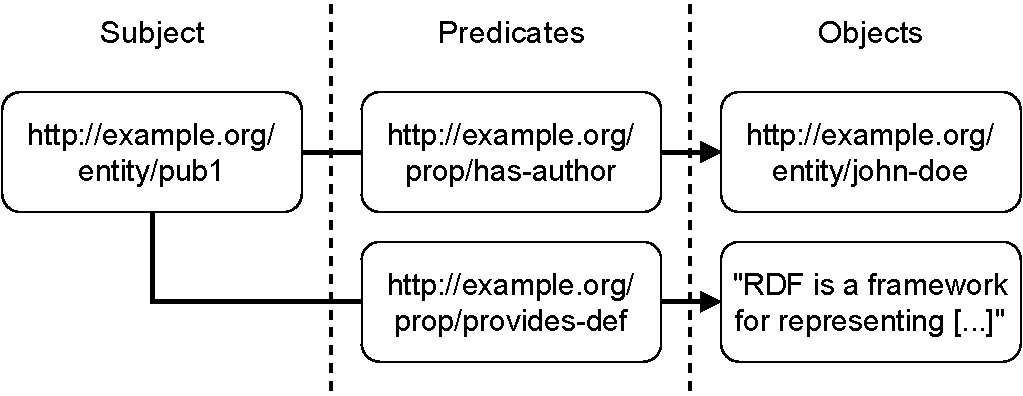
\includegraphics[max width=0.7\columnwidth]{/tex/example-basic/figures/triple_example}
\caption{A simple exemplary knowledge graph consisting of two RDF triples. The upper triple provides contextual information, the lower triple contentual information of the publication \emph{{pub1}}. All non-literal triple members are identified using IRIs. (Figure and caption adopted from~\cite{Martin21}.)}
\label{fig:contentual-contextual}
\end{figure}
% RDFtex Figure Import End
\Cref{fig:contentual-contextual} shows an imported figure.

\subsection{Software Import}

% RDFtex Software Import Start
\begin{software}
Prot{\'{e}}g{\'{e}}-2000~\cite{DBLP:conf/amia/NoyCFKTVM03}\\
Available at: \url{https://protege.stanford.edu}\\
Description: ``Prot\'{e}g\'{e}-2000 is an open-source tool that assists users in the construction of large electronic knowledge bases. It has an intuitive user interface that enables developers to create and edit domain ontologies."~\cite{DBLP:conf/amia/NoyCFKTVM03}
\label{software:protege}
\end{software}
% RDFtex Software Import End
\Cref{software:protege} shows an imported software.


